\documentclass[journal,12pt,onecolumn]{IEEEtran}
\usepackage{cite}
\usepackage{graphicx}
\usepackage{amsmath,amssymb,amsfonts,amsthm}
\usepackage{algorithmic}
\usepackage{graphicx}
\usepackage{textcomp}
\usepackage{xcolor}
\usepackage{txfonts}
\usepackage{listings}
\usepackage{enumitem}
\usepackage{mathtools}
\usepackage{gensymb}
\usepackage{comment}
\usepackage[breaklinks=true]{hyperref}
\usepackage{tkz-euclide} 
\usepackage{listings}
\usepackage{gvv}                                        
%\def\inputGnumericTable{}                                 
\usepackage[latin1]{inputenc} 
\usetikzlibrary{arrows.meta, positioning}
\usepackage{xparse}
\usepackage{color}                                            
\usepackage{array}                                            
\usepackage{longtable}                                       
\usepackage{calc}                                             
\usepackage{multirow}
\usepackage{multicol}
\usepackage{hhline}                                           
\usepackage{ifthen}                                           
\usepackage{lscape}
\usepackage{tabularx}
\usepackage{array}
\usepackage{float}
\usepackage{caption}
\usepackage{subcaption}
\newtheorem{theorem}{Theorem}[section]
\newtheorem{problem}{Problem}
\newtheorem{proposition}{Proposition}[section]
\newtheorem{lemma}{Lemma}[section]
\newtheorem{corollary}[theorem]{Corollary}
\newtheorem{example}{Example}[section]
\newtheorem{definition}[problem]{Definition}
\newcommand{\BEQA}{\begin{eqnarray}}
\newcommand{\EEQA}{\end{eqnarray}}
\usepackage{float}
%\newcommand{\define}{\stackrel{\triangle}{=}}
\theoremstyle{remark}
\usepackage{circuitikz}
\usepackage{tikz}

\title{IN  INSTRUMENTATION ENGINEERING}
\author{EE25BTECH11031- Sai Sreevallabh}

\author{Sai Sreevallabh - ee25btech11031}

\begin{document}

\maketitle

\begin{enumerate}

% Q1
\item Despite his initial hesitation, Rehman's \rule{1.5cm}{0.4pt} to contribute to the success of the project never wavered.\\
Select the most appropriate option to complete the sentece. 
\par\hfill{\brak{\text{GATE IN 2025}}}
\begin{enumerate}
\begin{multicols}{4}
\item ambivalence
\item satisfaction
\item resolve
\item revolve
\end{multicols}
\end{enumerate}

% Q2
\item Bird: Nest :: Bee : \rule{1.5cm}{0.4pt}\\
Select the correct option to complete the analogy.
\par\hfill{\brak{\text{GATE IN 2025}}}
\begin{enumerate}
\begin{multicols}{4}
\item Kennel
\item Hammock
\item Hive
\item Lair
\end{multicols}
\end{enumerate}

% Q3
\item If $P e^x = Q e^{-x}$ for all real values of $x$, which one of the following statements is true?
\par\hfill{\brak{\text{GATE IN 2025}}}
\begin{enumerate}
\begin{multicols}{2}
\item $P = Q = 0$
\item $P = Q = 1$
\item $P = 1, \; Q = -1$
\item $\frac{P}{Q} = 0$
\end{multicols}
\end{enumerate}

% Q4
\item The paper as shown in \figref{4} is folded to make a cube where each square corresponds to a particular face of the cube. Which one of the following options correctly represents the cube?
\par\hfill{\brak{\text{GATE IN 2025}}}
\begin{figure}[H]
\centering
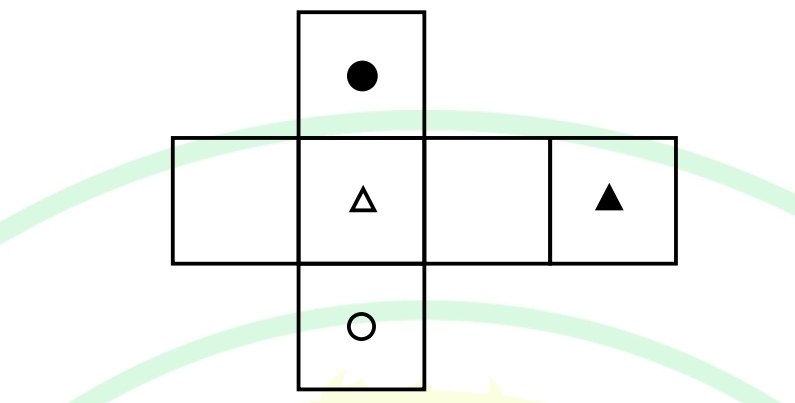
\includegraphics[width=0.4\columnwidth]{Figs/Q-4.jpg}
\caption{Outline of Cube}
\label{4}
\end{figure}
\begin{enumerate}
\begin{multicols}{2}
    \item 
    \begin{figure}[H]
        \centering
        
\includegraphics[width=0.2\columnwidth]{Figs/Q-4(a).png}
    \end{figure}
    
    \item 
    \begin{figure}[H]
        \centering
        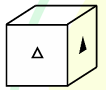
\includegraphics[width=0.2\columnwidth]{Figs/Q-4(b).png}
    \end{figure}

    \item 
    \begin{figure}[H]
        \centering
        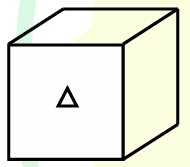
\includegraphics[width=0.2\columnwidth]{Figs/Q-4(c).png}
    \end{figure}

    \item 
    \begin{figure}[H]
        \centering
        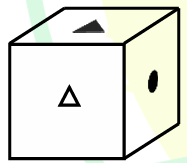
\includegraphics[width=0.2\columnwidth]{Figs/Q-4(d).png}
    \end{figure}
    
\end{multicols}
\end{enumerate}

% Q5
\item Let $p_1$ and $p_2$ denote two arbitrary prime numbers. Which one of the following statements is correct for all values of $p_1$ and $p_2$?
\par\hfill{\brak{\text{GATE IN 2025}}}
\begin{enumerate}
\begin{multicols}{2}
\item $p_1 + p_2$ is not a prime number.
\item $p_1 p_2$ is not a prime number.
\item $p_1 + p_2 + 1$ is a prime number.
\item $p_1 p_2 + 1$ is a prime number.
\end{multicols}
\end{enumerate}

% Q6
\item Based only on the conversation below, identify the logically correct inference:\\

``Even if I had known that you were in the hospital, I would not have gone there to see you", Ramya told Josephine.
\par\hfill{\brak{\text{GATE IN 2025}}}
\begin{enumerate}
\item Ramya knew that Josephine was in the hospital.
\item Ramya did not know that Josephine was in the hospital.
\item Ramya and Josephine were once close friends; but now, they are not.
\item Josephine was in the hospital due to an injury to her leg.
\end{enumerate}

% Q7
\item If IMAGE and FIELD are coded as FHBNJ and EMFJG respectively, then which one among the given options is the most appropriate code for BEACH?
\par\hfill{\brak{\text{GATE IN 2025}}}
\begin{enumerate}
\begin{multicols}{2}
\item CEADP
\item IDBFC
\item JGIBC
\item IBCEC
\end{multicols}
\end{enumerate}

% Q8
\item Which one of the following options is correct for the given data in the table? 
\par\hfill{\brak{\text{GATE IN 2025}}}
\begin{table}[H]
    \centering
    \begin{tabular}[12pt]{ |c| c| c| c| }
\hline
$\beta$ & Airplane A & Airplane B & Airplane C \\
\hline
$\beta = -5\,\mathrm{deg}$ & $-0.030$ & $-0.025$ & $0.040$\\
\hline
$\beta = 0\,\mathrm{deg}$ & $0$ & $0$ & $0$ \\
\hline
$\beta = 5\,\mathrm{deg}$ & $0.030$ & $0.025$ & $-0.040$\\
\hline
\end{tabular}
 
\end{table}
\begin{enumerate}
\item $X\brak{i} = X\brak{i-1} + I\brak{i}; \; Y\brak{i} = Y\brak{i-1} I\brak{i}, \; i>0$
\item $X\brak{i} = X\brak{i-1} I\brak{i}; \; Y\brak{i} = Y\brak{i-1} + I\brak{i}, \; i>0$
\item $X\brak{i} = X\brak{i-1} I\brak{i}; \; Y\brak{i} = Y\brak{i-1} I\brak{i}, \; i>0$
\item $X\brak{i} = X\brak{i-1} + I\brak{i}; \; Y\brak{i} = Y\brak{i-1} I\brak{i-1}, \; i>0$
\end{enumerate}

% Q9
\item In \figref{9}, PQRS is a square of side $2 \, \text{cm}$ and PLMN is a rectangle. The corner L is on QR. Side MN passes through S. Find the area of PLMN.\\
Note: the figure is representative. \par\hfill{\brak{\text{GATE IN 2025}}}
\begin{figure}[H]
\centering
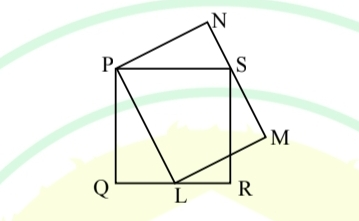
\includegraphics[width=0.4\columnwidth]{Figs/Q-9.jpg}
\caption{Diagram for Question-9}
\label{9}
\end{figure}
\begin{enumerate}
\begin{multicols}{4}
\item $2\sqrt{2}$
\item $2$
\item $8$
\item $4$
\end{multicols}
\end{enumerate}

% Q10
\item \figref{10} shows a river system with 7 segments P, Q, R, S, T, U, and V. It splits the land into 5 land zones, marked Z1, Z2, Z3, Z4, and Z5.We need to connect these zones using the least number of bridges. Out of the followinn options, which one is correct?\\
Note: THe figure shown is representative. \par\hfill{\brak{\text{GATE IN 2025}}}
\begin{figure}[H]
\centering
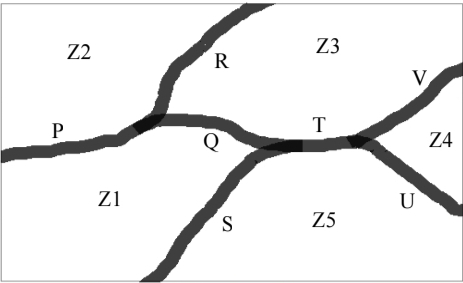
\includegraphics[width=0.4\columnwidth]{Figs/Q-10.jpg}
\caption{Division into Zones}
\label{10}
\end{figure}
\begin{enumerate}
\begin{multicols}{2}
\item Bridges on P, Q, and T
\item Bridges on P, Q, S, and T
\item Bridges on Q, R, T, and V
\item Bridges on P, Q, S, U, and V
\end{multicols}
\end{enumerate}

% Q11
\item A $2n \times 2n$ matrix $A=\myvec{a_{ij}}$ has \\

$$
a_{ij} = 
\begin{cases}
    \beta & if \brak{i+j} \text{is odd},\\
    -\beta & if \brak{i+j} \text{is even},
\end{cases}$$
where $n$ is any integer greater than 2 and $\beta$ is any non-zero real number. Rank of A is
\par\hfill{\brak{\text{GATE IN 2025}}}
\begin{enumerate}
\begin{multicols}{2}
\item $1$
\item $2$
\item $n$
\item $2n$
\end{multicols}
\end{enumerate}

% Q12
\item The solution of $\frac{dy}{dx} = 9\frac{x}{y}$ represents
\par\hfill{\brak{\text{GATE IN 2025}}}
\begin{enumerate}
\begin{multicols}{2}
\item a hyperbola
\item a parabola
\item an ellipse
\item a circle
\end{multicols}
\end{enumerate}

% Q13
\item The working principle of a hand-held metal detector most widely used by security personnel for human frisking is based on the principle of
\par\hfill{\brak{\text{GATE IN 2025}}}
\begin{enumerate}
\item change in reluctance of iron core in presence of a metallic object
\item change in conductance of iron core in presence of a metallic object
\item electric field induced by a metallic object
\item eddy current generation in a metallic object
\end{enumerate}


% Q14
\item The primary coil of a linear variable differential transformer (LVDT) is supplied with AC voltage as shown in \figref{14}. The secondary coils are connected in series opposition and the output is measured using a true RMS voltmeter.  
The displacement $x$ of the core is indicated in mm on a linear scale. At the null position $x = 0$, the voltmeter reads $0 \, V$. If the voltmeter reads $0.2 \, V$ for a displacement of $x = +2 \, \text{mm}$, then for a displacement of $x = -3 \, \text{mm}$, the voltmeter reading, in $V$, is \par\hfill{\brak{\text{GATE IN 2025}}}

\begin{figure}[H]
    \centering
    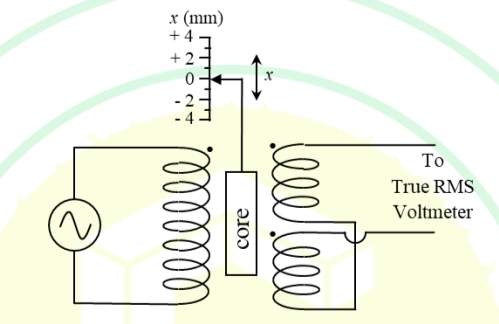
\includegraphics[width=0.5\columnwidth]{Figs/Q-14.jpg}
    \caption{Linear Variable Differential Transformer}
    \label{14}
\end{figure}

\begin{enumerate}
\begin{multicols}{2}
\item $-0.3$
\item $-0.1$
\item $0.3$
\item $0.5$
\end{multicols}
\end{enumerate}

% Q15  
\item In the force transducer shown in \figref{15(a)}, four identical strain gauges $S_1$, $S_2$, $S_3$, and $S_4$ are mounted on a cantilever at equal distance from its base. $S_1$ and $S_2$ are mounted on the top surface and $S_3$ and $S_4$ are mounted on the bottom surface.  
These strain gauges are to be connected to form a Wheatstone bridge consisting of arms 
A, B, C, D, as shown in \figref{15(b)}. From the following options, the correct order to maximize the
measurement sensitivity is \par\hfill{\brak{\text{GATE IN 2025}}}
\begin{figure}[H]
\centering
\begin{subfigure}{.5\columnwidth}
  \centering
  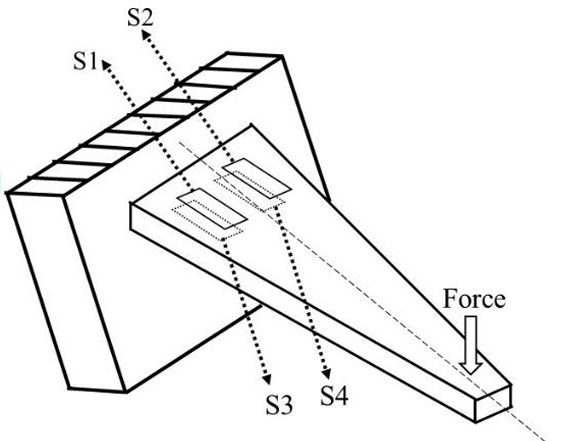
\includegraphics[width=.6\columnwidth]{Figs/Q-15(a).png}
  \caption{Force Transducer}
  \label{15(a)}
\end{subfigure}%
\begin{subfigure}{.5\columnwidth}
  \centering
  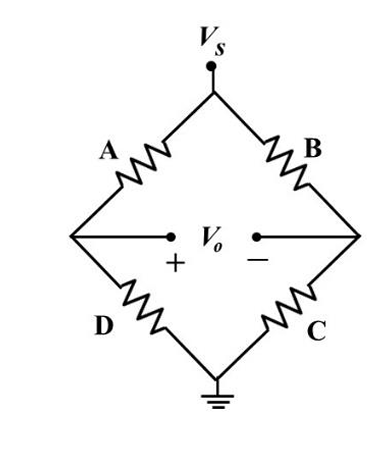
\includegraphics[width=.4\columnwidth]{Figs/Q-15(b).png}
  \caption{Wheatstone Bridge}
  \label{15(b)}
\end{subfigure}
\caption{Diagrams for Question-15}
\label{15}
\end{figure}
\begin{enumerate}
\begin{multicols}{2}
\item A$\to S_1$, B$\to S_2$, C$\to S_4$, D$\to S_3$
\item A$\to S_1$, B$\to S_4$, C$\to S_3$, D$\to S_2$
\item A$\to S_1$, B$\to S_2$, C$\to S_3$, D$\to S_4$
\item A$\to S_1$, B$\to S_4$, C$\to S_2$, D$\to S_3$
\end{multicols}
\end{enumerate}


% Q16
\item Let a continuous-time signal be $x\brak{t} = e^{j9t} + e^{j5t}$, where $j=\sqrt{-1}$ and $t$ is in seconds.  
The fundamental period of magnitude of $x\brak{t}$, in seconds, is
\par\hfill{\brak{\text{GATE IN 2025}}}
\begin{enumerate}
\begin{multicols}{4}
\item $\pi$
\item $\frac{\pi}{2}$
\item $\frac{\pi}{5}$
\item $\frac{\pi}{9}$
\end{multicols}
\end{enumerate}

% Q17
\item The minimized expression of the Boolean function $Y\brak{P,Q,R}$ implemented by the multiplexer (MUX)
circuit shown in \figref{17} is \par\hfill{\brak{\text{GATE IN 2025}}}
\begin{figure}[H]
    \centering
    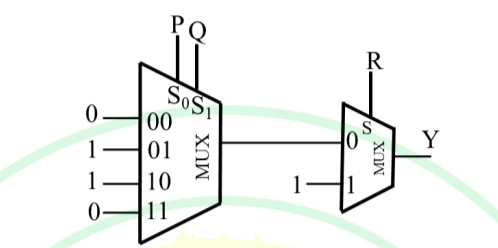
\includegraphics[width=0.5\columnwidth]{Figs/Q-17.jpg}
    \caption{Multiplexer}
    \label{17}
\end{figure}
\begin{enumerate}
\begin{multicols}{2}
\item $Y = R + \brak{P\oplus Q}$
\item $Y = R(P \oplus Q)$
\item $Y = R + \overline{\brak{P\oplus Q}}$
\item $Y = R \oplus (P \oplus Q)$
\end{multicols}
\end{enumerate}

% Q18
\item The $4$-bit signed $2$'s complement form of $\brak{5}_{10} + \brak{5}_{10}$ is \par\hfill{\brak{\text{GATE IN 2025}}}
\begin{enumerate}
\begin{multicols}{4}
\item $\brak{-6}_{10}$
\item $\brak{-7}_{10}$
\item $\brak{-5}_{10}$
\item $\brak{-8}_{10}$
\end{multicols}
\end{enumerate}

% Q19
\item An infinite sheet of uniform charge $\rho_s = 10 \, C/m^2$ is placed on $z=0$ plane.  
The medium surrounding the sheet has a relative permittivity of $10$.  
The electric flux density, in $C/m^2$, at a point $P\brak{0,0,5}$ is\\
Note: $\hat{a}$, $\hat{b}$ and $\hat{c}$ are unit vectors along the $x, y,$ and $z$ directions respectively. \par\hfill{\brak{\text{GATE IN 2025}}}
\begin{enumerate}
\begin{multicols}{4}
\item $5 \, \hat{c}$
\item $0.25 \, \hat{c}$
\item $10 \, \hat{c}$
\item $0.5 \, \hat{c}$
\end{multicols}
\end{enumerate}

% Q20
\item For the ideal opamp based circuit shown in \figref{20}, the ratio $\frac{V}{I}$ is \par\hfill{\brak{\text{GATE IN 2025}}}
\begin{figure}[H]
    \centering
    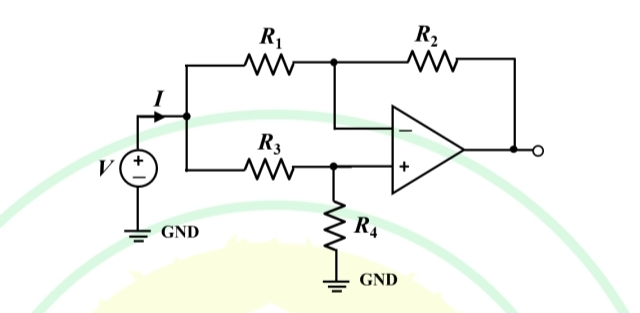
\includegraphics[width=0.5\columnwidth]{Figs/Q-20.jpg}
    \caption{Circuit Diagram for Question-20}
    \label{20}
\end{figure}
\begin{enumerate}
\begin{multicols}{4}
\item $\brak{\frac{R_3 + R_4}{R_1 + R_3}}R_1$
\item $\brak{\frac{R_2 + R_4}{R_3+R_1}}R_3$
\item $R_1+R_3$
\item ${R_3+R_4}$
\end{multicols}
\end{enumerate}

% Q21
\item In a single-phase AC circuit, the power consumed by load resistance $R_L$ for an excitation $V_s$ is measured using a wattmeter. The same wattmeter is connected in two different topologies, Topology-A and Topology-B, as shown in \figref{21}. Different branch currents and voltage drops are also marked in the figure.Among the following options, the condition that ensures low error in the wattmeter reading for both is
\par\hfill{\brak{\text{GATE IN 2025}}}
\begin{figure}[H]
    \centering
    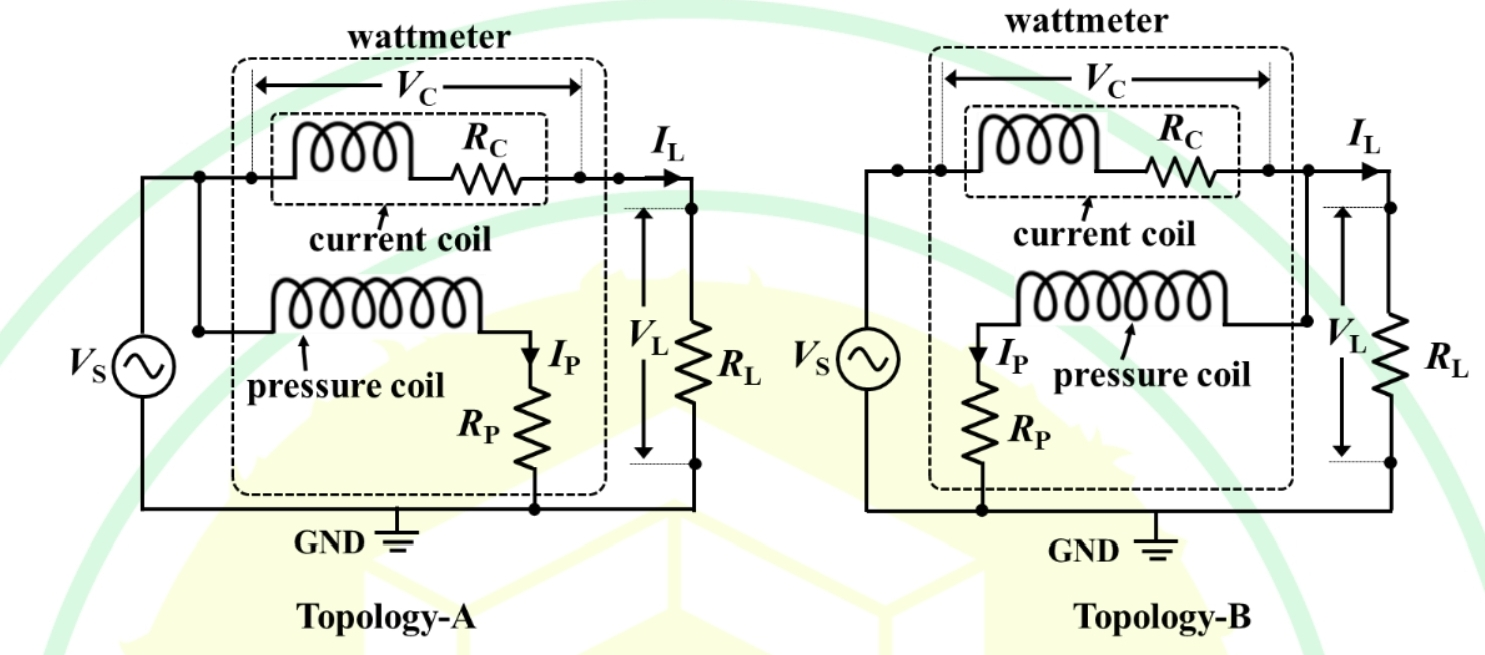
\includegraphics[width=0.7\columnwidth]{Figs/Q-21.jpg}
    \caption{Topologies A and B}
    \label{21}
\end{figure}
\begin{enumerate}
\item $V_L \gg V_c$ for Topology-A and $I_L \gg I_P$ for Topology-B
\item $V_L \gg V_c$ for Topology-A and $I_L \ll I_P$ for Topology-B
\item $V_L \ll V_c$ for Topology-A and $I_L \ll I_P$ for Topology-B
\item $V_L \ll V_c$ for Topology-A and $I_L \approx I_P$ for Topology-B
\end{enumerate}

% Q22
\item Match the following sensors with their applications:  
\begin{table}[H]
    \centering
    \begin{table}[h!]
\small
\setlength{\tabcolsep}{4pt}
\renewcommand{\arraystretch}{0.9}
\centering
\begin{tabular}{|c|c|c|p{1.8cm}|p{2.5cm}|c|}
\hline
Q. No & Type & Section & Key & Marks \\
\hline
1  & MCQ & GA & C         & 1 \\
\hline
2  & MCQ & GA & A         & 1 \\
\hline
3  & MCQ & GA & A         & 1 \\
\hline
4  & MCQ & GA & A         & 1 \\
\hline
5  & MCQ & GA & D         & 1 \\
\hline
6  & MCQ & GA & D         & \textbf{2} \\
\hline
7  & MCQ & GA & B         & 2 \\
\hline
8  & MCQ & GA & C         & 2 \\
\hline
9  & MCQ & GA & B         & 2 \\
\hline
10 & MCQ & GA & C         & 2 \\
\hline
11 & MCQ & EY & D         & 1 \\
\hline
12 & MCQ & EY & D         & 1 \\
\hline
13 & MCQ & EY & A; D      & 1 \\
\hline
14 & MCQ & EY & B         & 1 \\
\hline
15 & NAT & EY & 7.99 : 8.10 & 1 \\
\hline
16 & MCQ & EY & B         & 1 \\
\hline
17 & MCQ & EY & C         & 1 \\
\hline
18 & MCQ & EY & D         & 1 \\
\hline
19 & NAT & EY & 9.9 : 10.1  & 1 \\
\hline
20 & MCQ & EY & C         & 1 \\
\hline
21 & MCQ & EY & B         & 1 \\
\hline
22 & MCQ & EY & A         & 1 \\
\hline
23 & MCQ & EY & D         & 1 \\
\hline
24 & MCQ & EY & B         & 1 \\
\hline
25 & MCQ & EY & A         & 1 \\
\hline
26 & MCQ & EY & C         & 2 \\
\hline
27 & MCQ & EY & D         & 2 \\
\hline
28 & MCQ & EY & C         & 2 \\
\hline
29 & MCQ & EY & D         & 2 \\
\hline
30 & MCQ & EY & B         & 2 \\
\hline
31 & MCQ & EY & A         & 2 \\
\hline
32 & MCQ & EY & C         & 2 \\
\hline
33 & MCQ & EY & A         & 2 \\
\hline
34 & MCQ & EY & B         & 2 \\
\hline
35 & MCQ & EY & A         & 2 \\
\hline
36 & MCQ & EY & A         & 2 \\
\hline
37 & MCQ & EY & C         & 2 \\
\hline
38 & MCQ & EY & A         & 2 \\
\hline
39 & NAT & EY & 0.17 : 0.19 & 2 \\
\hline
40 & MCQ & EY & A         & 2 \\
\hline
41 & MCQ & EY & B         & 2 \\
\hline
42 & MCQ & EY & B         & 2 \\
\hline
43 & MCQ & EY & A         & 2 \\
\hline
44 & MCQ & EY & D         & 2 \\
\hline
45 & MCQ & EY & B         & 2 \\
\hline
46 & MCQ & EY & A         & 2 \\
\hline
47 & NAT & EY & 0.175 : 0.20 & 2 \\
\hline
48 & MCQ & EY & A         & 2 \\
\hline
49 & NAT & EY & 0.49 : 0.51  & 2 \\
\hline
50 & MCQ & EY & B         & 2 \\
\hline
51 & MCQ & EY & A         & 2 \\
\hline
52 & MCQ & EY & C         & 2 \\
\hline
53 & NAT & EY & 1660 : 1700 & 2 \\
\hline
54 & NAT & EY & 0.45 : 0.55 & 2 \\
\hline
55 & MCQ & EY & A         & 2 \\
\hline
\end{tabular}
\caption{GATE 2016 EY Answer Key Summary}
\end{table}
\end{table}
\par\hfill{\brak{\text{GATE IN 2025}}}
\begin{enumerate}
\begin{multicols}{2}
\item P-II, Q-III, R-I, S-IV
\item P-II, Q-IV, R-III, S-I
\item P-III, Q-IV, R-II, S-I
\item P-III, Q-IV, R-I, S-II
\end{multicols}
\end{enumerate}

% Q23
\item A $3\frac{1}{2}$ digit digital voltmeter has accuracy $\pm\brak{0.5\% + 1}$. If used to measure $10\, V$ DC, the error in the measurement would be\\
Note: Accuracy of the digital voltmeter is expressed as $\pm$(\%of reading + digit). 
\begin{enumerate}
\begin{multicols}{4}
\item $\pm 0.4\%$
\item $\pm 1.5\%$
\item $\pm 0.6\%$
\item $\pm 1\%$
\end{multicols}
\end{enumerate}

% Q24
\item The circuit shown in \figref{24(a)} can be represented using its T-model shown in \figref{24(b)}. The values of the inductances $L_1,L_2$ and $L_3$. in equivalent T-model are \par\hfill{\brak{\text{GATE IN 2025}}}
\begin{figure}[H]
\centering
\begin{subfigure}{.5\columnwidth}
  \centering
  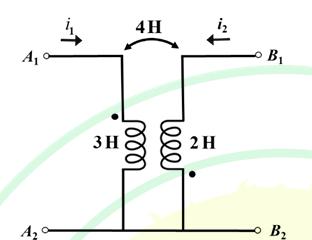
\includegraphics[width=.6\columnwidth]{Figs/Q-24(a).png}
  \caption{Given Circuit}
  \label{24(a)}
\end{subfigure}%
\begin{subfigure}{.5\columnwidth}
  \centering
  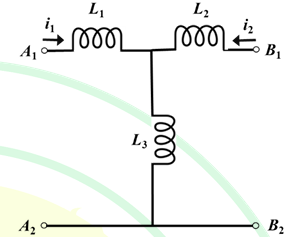
\includegraphics[width=.6\columnwidth]{Figs/Q-24(b).png}
  \caption{T-model of given circuit}
  \label{24(b)}
\end{subfigure}
\caption{Diagrams for Question-24}
\label{24}
\end{figure}
\begin{enumerate}
\begin{multicols}{2}
\item $L_1 = 7H,\; L_2=6H,\; L_3=-4H$
\item $L_1 = -1H,\; L_2=-2H,\; L_3=4H$
\item $L_1 = 3H,\; L_2=2H,\; L_3=9H$
\item $L_1 = 1H,\; L_2=-2H,\; L_3=-4H$
\end{multicols}
\end{enumerate}

%25
\item Three parallel admittances $Y_a=-j0.2\,S$, $Y_b=0.3\,S$, and $Y_c=j0.4\,S$ connected in parallel with a voltage source $V=10\angle 45\degree$ V, draw a total current $I_s$ from the source. The currents flowing through each of these admittances are $I_a, I_b$ and $I_c$, respectively. Let $I=I_a+I_b$. The phase relation between $I$ and $I_s$ is
\par\hfill{\brak{\text{GATE IN 2025}}}
\begin{enumerate}
\begin{multicols}{2}
\item $I$ leads $I_s$ by $19.44\degree$
\item $I$ lags $I_s$ by $19.44\degree$
\item $I$ leads $I_s$ by $33.69\degree$
\item $I$ lags $I_s$ by $33.69\degree$
\end{multicols}
\end{enumerate}


%26
\item An oscilloscope has an input resistance of $1\,M\ohm$. A 10$X$ passive attenuating probe is connected to it. The effective input resistance, in $M\ohm$, seen into the probe tip is \par\hfill{\brak{\text{GATE IN 2025}}}
\begin{enumerate}
\begin{multicols}{4}
\item $0.9$
\item $9.1$
\item $10$
\item $11$
\end{multicols}
\end{enumerate}

%27
\item For the transfer function 
$$G\brak=\frac{2s-1}{s^3+5s^2+3s+22}$$
the number of zeros lying in the left half $s$-plane is \par\hfill{\brak{\text{GATE IN 2025}}}
\begin{enumerate}
\begin{multicols}{4}
\item $0$
\item $1$
\item $2$
\item $3$
\end{multicols}
\end{enumerate}


%28
\item Consider the control system block diagram. The loop transfer $G\brak{s}H\brak{s}$ does not have any pole on the $j\omega$-axis. The counterclockwise contour with infinite radius, as shown in \figref{28(b)} encircles two poles of $G\brak{s}H\brak{s}$. The correct condition for closed-loop stability is \par\hfill{\brak{\text{GATE IN 2025}}}
\begin{figure}[H]
\centering
\begin{subfigure}{.5\columnwidth}
  \centering
  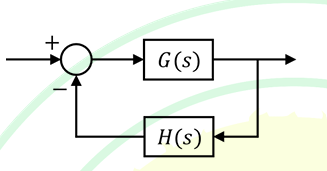
\includegraphics[width=.4\columnwidth]{Figs/Q-28(a).png}
  \caption{Control system block diagram}
  \label{28(a)}
\end{subfigure}
\begin{subfigure}{.5\columnwidth}
  \centering
  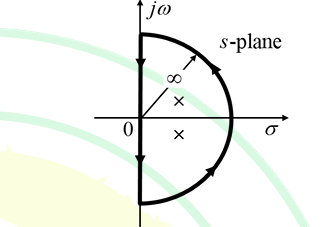
\includegraphics[width=.4\columnwidth]{Figs/Q-28(b).png}
  \caption{Poles encircled by the contour}
  \label{28(b)}
\end{subfigure}
\caption{Diagrams for Question-28}
\label{fig:test}
\end{figure}
\begin{enumerate}
\item The locus of $G\brak{s}H\brak{s}$ should encircle the origin twice in counter-clockwise direction
\item The locus of $1+G\brak{s}H\brak{s}$ should encircle the origin twice in clockwise direction
\item The locus of $G\brak{s}H\brak{s}$ should encircle the $-1+j0$ point twice in counter-clockwise direction
\item The locus of $1+G\brak{s}H\brak{s}$ should encircle the $-1+j0$ point twice clockwise direction. 
\end{enumerate}


%29
\item A Boolean function $X$ is given as $X=\bar A\bar B+\bar A\bar C$. The reduced form of $\bar X$ is \par\hfill{\brak{\text{GATE IN 2025}}}
\begin{enumerate}
\begin{multicols}{4}
\item $\bar A+\bar B+\bar C$
\item $A+BC$
\item $\bar{A}+\bar B+C$
\item $B+AC$
\end{multicols}
\end{enumerate}


%30
\item A $60$ V DC source with internal resistance $R_{int}=0.5\ohm$ is connected through a switch to a pair of infinitely long rails separated by $l=1$ m as shown in \figref{30}. THe rails are placed in a constant uniform magnetic field of flux density $B=0.5$ T  directed into the page. A conducting bar placed on rails moves freely. At the instant of closing the switch, the force induced on the bar is\\
Note: Assume there is no friction between the bar and the rails. The resistances of the conducting bar and the rails are zero. \par\hfill{\brak{\text{GATE IN 2025}}}
\begin{figure}[H]
\centering
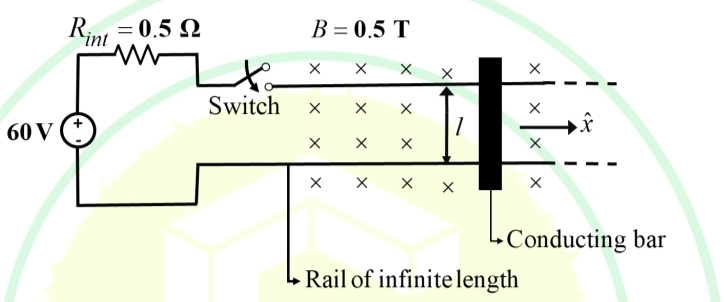
\includegraphics[width=0.5\columnwidth]{Figs/Q-30.jpg}
\caption{Diagram for Question-30}
\label{30}
\end{figure}
\begin{enumerate}
\begin{multicols}{2}
\item $60$ N in the direction of $\hat{x}$
\item $60$ N opposite to the direction of $\hat{x}$
\item $120$ N in the direction of $\hat{x}$
\item $120$ N opposite to the direction of $\hat{x}$
\end{multicols}
\end{enumerate}


%31
\item The circuits mentioned below are realized using ideal opamp. Among these, the circuit(s) performing non-linear operation on the input signal is/are \par\hfill{\brak{\text{GATE IN 2025}}}
\begin{enumerate}
\begin{multicols}{2}
\item Instrumentation amplifier
\item Schmitt trigger
\item Logarithmic amplifier
\item Precision rectifier
\end{multicols}
\end{enumerate}


%32
\item If one of the eigenvectors of the matrix 
$A=\myvec{-1 & -1\\ x & -4}$
is along direction of $\myvec{\alpha \\ 2\alpha}$, where $\alpha$ is any non-zero real number, then the value of $x$ is \rule{1.5cm}{0.4pt}.(integer) \par\hfill{\brak{\text{GATE IN 2025}}}


%33
\item Consider the function $f\brak{z}=\frac{2z+1}{z^2-z}$, where $z$ is a complex variable. The sum of the residues at singular points of $f\brak{z}$ is \rule{1.5cm}{0.4pt}. (integer) \par\hfill{\brak{\text{GATE IN 2025}}}


%34
\item A dual-slope ADC has fixed integration time of $100$ ms. The reference voltage is $-5$ V. The time taken by the ADC to measure input $1.25$ V is \rule{1.5cm}{0.4pt} ms. (rounded off to the nearest integer) \par\hfill{\brak{\text{GATE IN 2025}}}
 

%35
\item In the circuit shown in \figref{35}, assume BJT in the circuit has very high $\beta$ and $V_{BE}=0.7$ V. The Zener diode has $V_z=4.7$ V. The current $I$ through the LED is \rule{1.5cm}{0.4pt} mA. \par\hfill{\brak{\text{GATE IN 2025}}}
\begin{figure}[H]
\centering
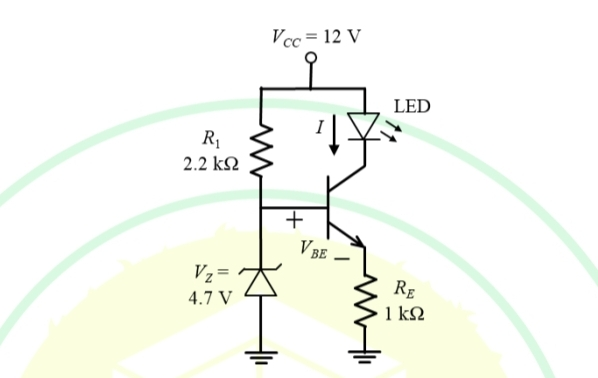
\includegraphics[width=0.5\columnwidth]{Figs/Q-35.jpg}
\caption{Circuit Diagram for Question-35}
\label{35}
\end{figure}


%36
\item The value of the surface integral 
$$\iint_S \brak{2x+z}\,dy\,dz + \brak{2x+z}\,dx\,dz + \brak{2z+y}\,dx\,dy$$
over the sphere $S \colon x^2 + y^2 + z^2 = 9$ is \par\hfill{\brak{\text{GATE IN 2025}}}
\begin{enumerate}
\begin{multicols}{4}
\item $72\pi$
\item $144\pi$
\item $36\pi$
\item $432\pi$
\end{multicols}
\end{enumerate}


%37
\item Newton-Raphson method is used to compute the inverse of the number $1.6$. Among the following options, the initial guess of the solution that results in non-convergence of the iterative process is \par\hfill{\brak{\text{GATE IN 2025}}}
\begin{enumerate}
\begin{multicols}{4}
\item $0.55$
\item $0.75$
\item $1.15$
\item $1.25$
\end{multicols}
\end{enumerate}


%38
\item The value of the integral
$\int_{-\pi}^{\pi} \brak{\cos^4 x + \cos^6 x}\,dx$
is \par\hfill{\brak{\text{GATE IN 2025}}}
\begin{enumerate}
\begin{multicols}{4}
\item $\tfrac{\pi}{2}$
\item $\tfrac{5\pi}{8}$
\item $\tfrac{11\pi}{8}$
\item $\tfrac{9\pi}{8}$
\end{multicols}
\end{enumerate}


%39
\item Let $y\sbrak{n} = \frac{1}{\alpha} y\sbrak{n-1} + x\sbrak{n}$, where $\alpha > 1$ and real, represent a difference equation of a causal discrete-time LTI system. The system is initially at rest. If $x\sbrak
n= \delta\sbrak{n-p}$ where $p>10$, the value of $y\sbrak{p+1}$ is \par\hfill{\brak{\text{GATE IN 2025}}}
\begin{enumerate}
\begin{multicols}{4}
\item $0$
\item $1$
\item $\frac{1}{\alpha}$
\item $\frac{1}{\alpha^2}$
\end{multicols}
\end{enumerate}


%40
\item The clock frequency of the digital circuit shown in \figref{40} is $12\,\text{MHz}$. The frequencies of the output $F$ corresponding to Control $=0$ and Control $=1$, respectively, are \par\hfill{\brak{\text{GATE IN 2025}}}
\begin{figure}[H]
\centering
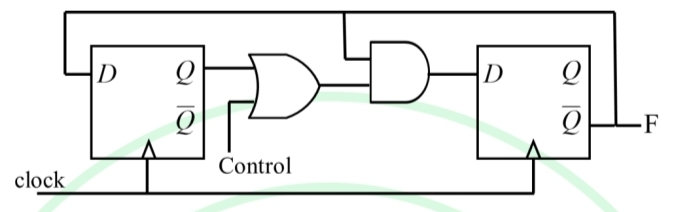
\includegraphics[width=0.5\columnwidth]{Figs/Q-40.jpg}
\caption{Digital Circuit for Question-40}
\label{40}
\end{figure}
\begin{enumerate}
\begin{multicols}{2}
\item $4\,\text{MHz}$ and $6\,\text{MHz}$
\item $6\,\text{MHz}$ and $4\,\text{MHz}$
\item $3\,\text{MHz}$ and $4\,\text{MHz}$
\item $3\,\text{MHz}$ and $6\,\text{MHz}$
\end{multicols}
\end{enumerate}


%41
\item A chopper amplifier shown in \figref{41} is designed to process a biomedical signal $v_{in}\brak{t}$ to generate conditioned output $v_{out}\brak{t}$. The signals $v_{in}\brak{t}$ and $v_{os}\brak{t}$ are band limited to $50\,\text{Hz}$ and $10\,\text{Hz}$ respectively. For the system to operate as a linear amplifier, choose the correct statement from the following options. \par\hfill{\brak{\text{GATE IN 2025}}}
\begin{figure}[H]
\centering
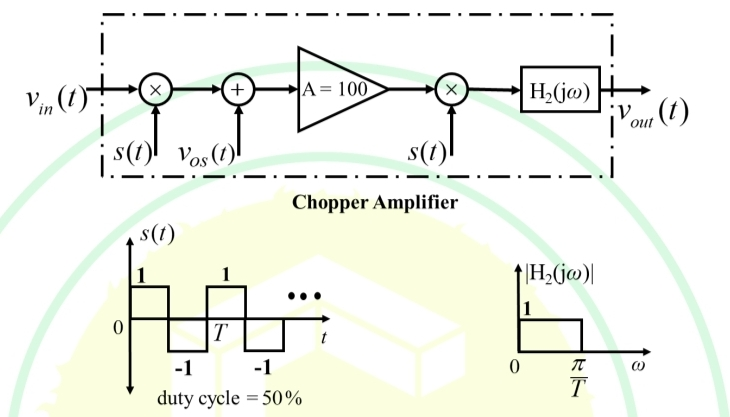
\includegraphics[width=0.7\columnwidth]{Figs/Q-41.jpg}
\caption{Diagram for Question-41}
\label{41}
\end{figure}
\begin{enumerate}
\item The minimum frequency of $s\brak{t}$ required is $100\,\text{Hz}$ and $v_{os}\brak{t}$ gets attenuated by the system
\item The minimum frequency of $s\brak{t}$ required is $100\,\text{Hz}$ and $v_{os}\brak{t}$ also gets amplified by the system by a factor $200$
\item The minimum frequency of $s\brak{t}$ required is $80\,\text{Hz}$ and $v_{os}\brak{t}$ gets attenuated by the system
\item The minimum frequency of $s\brak{t}$ required is $80\,\text{Hz}$ and $v_{os}\brak{t}$ also gets amplified by the system by a factor $\tfrac{200}{\pi}$
\end{enumerate}


%42
\item An $8$-bit microprocessor has $16$-bit address bus $A_{15}$-$A_0$ where $A_0$ is the LSB. As shown in \figref{42(a)} it has a pre-installed $4$ KB ROM whose starting address is 0000H. The processor needs to be upgraded by adding a $16$ KB RAM as shown in \figref{42(b)}. The address range for the newly added RAM is \par\hfill{\brak{\text{GATE IN 2025}}}
\begin{figure}[H]
\centering
\begin{subfigure}{.5\columnwidth}
  \centering
  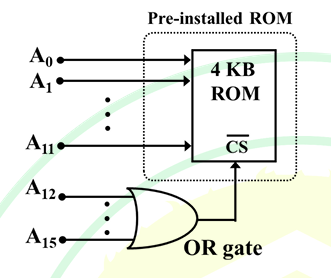
\includegraphics[width=.6\columnwidth]{Figs/Q-42(a).png}
  \caption{Pre-installed ROM}
  \label{42(a)}
\end{subfigure}%
\begin{subfigure}{.5\textwidth}
  \centering
  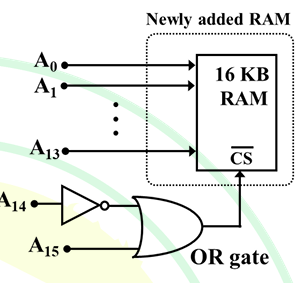
\includegraphics[width=.6\columnwidth]{Figs/Q-42(b).png}
  \caption{Newly Added RAM}
  \label{42(b)}
\end{subfigure}
\caption{Diagrams for Question-42}
\label{42}
\end{figure}
\begin{enumerate}
\begin{multicols}{2}
\item $1000$H - $4$FFFH
\item $3000$H - $6$FFFH
\item $4000$H - $7$FFFH
\item $8000$H - BFFFH
\end{multicols}
\end{enumerate}


%43
\item A $3$-bit DAC is implemented using ideal opamp and switches as shown in \figref{43}. Each of the switches gets closed when its corresponding digital input is at logic $1$. For a digital input $110$, the resistance $R_{in}$ seen from the reference source and the current $I$ are \par\hfill{\brak{\text{GATE IN 2025}}}
\begin{figure}[H]
\centering
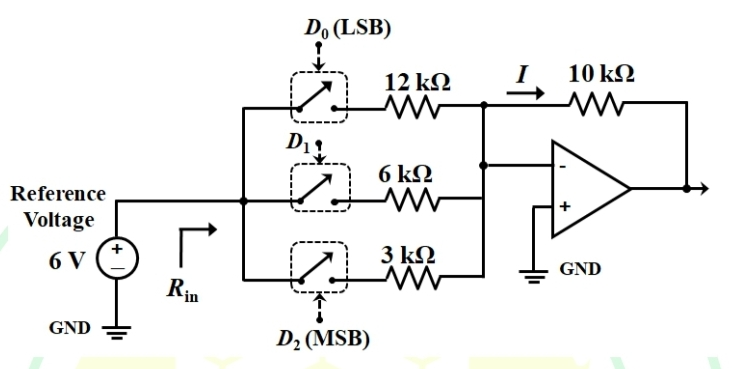
\includegraphics[width=0.6\columnwidth]{Figs/Q-43.jpg}
\caption{Arrangement of OpAmp and Switches}
\label{43}
\end{figure}
\begin{enumerate}
\item $R_{in}=2\,k\ohm$, $I=3\,\text{mA}$
\item $R_{in}=12\,k\ohm$, $I=0.5\,\text{mA}$
\item $R_{in} = \infty$, $I=1\,\text{mA}$
\item $R_{in} = \infty$, $I=3\,\text{mA}$
\end{enumerate}


%44
\item Power consumed by a three-phase balanced load is measured using two-wattmeter method. The per-phase average power drawn is $30\,\text{kW}$ at $\frac{\sqrt{3}}{2}$ lagging power factor. The readings of the wattmeters will be \par\hfill{\brak{\text{GATE IN 2025}}}
\begin{enumerate}
\begin{multicols}{2}
\item $15\,\text{kW}$ and $15\,\text{kW}$
\item $22.5\,\text{kW}$ and $7.5\,\text{kW}$
\item $60\,\text{kW}$ and $30\,\text{kW}$
\item $45\,\text{kW}$ and $45\,\text{kW}$
\end{multicols}
\end{enumerate}


%45
\item The bridge circuit shown in \figref{45(a)} can be equivalently represented as shown in \figref{45(b)}. The values of $R_1, R_2$, and $V_c$ in the equivalent circuit are \par\hfill{\brak{\text{GATE IN 2025}}}
\begin{figure}[H]
\centering
\begin{subfigure}{.5\columnwidth}
  \centering
  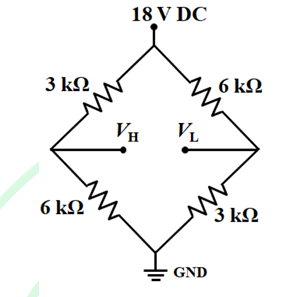
\includegraphics[width=.4\columnwidth]{Figs/Q-45(a).png}
  \caption{Bridge Circuit}
  \label{45(a)}
\end{subfigure}
\begin{subfigure}{.5\textwidth}
  \centering
  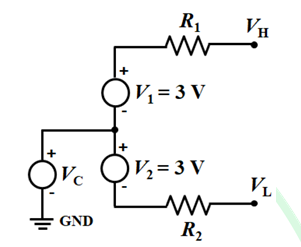
\includegraphics[width=.4\columnwidth]{Figs/Q-45(b).png}
  \caption{Equivalent Circuit}
  \label{45(b)}
\end{subfigure}
\caption{Diagrams for Question-45}
\label{45}
\end{figure}
\begin{enumerate}
\begin{multicols}{2}
\item $R_1=6\,k\ohm$, $R_2=3\,k\ohm$, $V_c=9\,V$
\item $R_1=3\,k\ohm$, $R_2=6\,k\ohm$, $V_c=4.5\,V$
\item $R_1=2\,k\ohm$, $R_2=2\,k\ohm$, $V_c=9\,V$
\item $R_1=2\,k\ohm$, $R_2=2\,k\ohm$, $V_c=4.5\,V$
\end{multicols}
\end{enumerate}


%46
\item A $2$-pole, $50$ Hz, $3$-phase induction motor supplies power to a certain load at $2970\,\text{rpm}$. The torque-speed curve of this machine follows a linear relationship between synchronous speed and 95\% of synchronous speed. Assume mechanical and stray losses to be $0$. If the load torque of the motor is doubled, the new operating speed (in rpm) is \par\hfill{\brak{\text{GATE IN 2025}}}
\begin{enumerate}
\begin{multicols}{4}
\item $2940$
\item $2812$
\item $2970$
\item $2850$
\end{multicols}
\end{enumerate}


%47
\item \figref{47} shows a closed-loop system with a plant $G\brak{s}=\tfrac{1}{s^2}$ and a lead compensator $C\brak{s}$. The compensator is designed to place the dominant closed-loop poles at $-1.5 \pm j\tfrac{\sqrt{27}}{2}$. From the following options, choose the phase lead that the compensator needs to contribute. \par\hfill{\brak{\text{GATE IN 2025}}}
\begin{figure}[H]
    \centering
    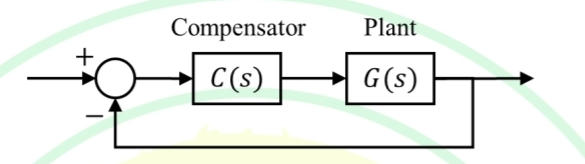
\includegraphics[width=0.5\columnwidth]{Figs/Q-47.jpg}
    \caption{Closed Loop system}
    \label{47}
\end{figure}
\begin{enumerate}
\begin{multicols}{4}
\item $30\degree$
\item $60\degree$
\item $90\degree$
\item $120\degree$
\end{multicols}
\end{enumerate}


%48
\item Let $f\brak{t}$ and $g\brak{t}$ represent continuous-time real-valued signals. If $h\brak{t}$ denotes cross-correlation between $f\brak{t}$ and $g\brak{-t}$, its continuous-time Fourier transform $H\brak{j\omega}$ equals  \\
Note: $F\brak{j\omega}$ and $G\brak{j\omega}$ denote the continuous-time Fourier transforms of $f\brak{t}$ and $g\brak{t}$ respectively. \par\hfill{\brak{\text{GATE IN 2025}}}
\begin{enumerate}
\begin{multicols}{2}
\item $F\brak{j\omega}G\brak{j\omega}$
\item $F\brak{-j\omega}G\brak{j\omega}$
\item $F\brak{j\omega}G\brak{-j\omega}$
\item $-F\brak{j\omega}G\brak{-j\omega}$
\end{multicols}
\end{enumerate}


%49
\item Choose the correct statement(s) regarding Cauchy's theorem on complex integration $\oint_C f\brak{z}dz$ where $C$ is a simple closed path and $D$ is simply connected domain.  \par\hfill{\brak{\text{GATE IN 2025}}}
\begin{enumerate}
\item Cauchy's theorem cannot be directly applied to conclude that $\oint_C \tfrac{1}{z^2}dz=0$ when $C$ is the unit circle.
\item If $f\brak{z}$ is analytic in $D$, then $\oint_C f\brak{z}dz=0$ for any simple closed path $C$ in $D$.
\item The function $f\brak{z}$ must be analytic in $D$ to conclude $\oint_C f\brak{z}dz=0$.
\item $\oint_C f\brak{z}dz \ne 0$ when $f\brak{z} = \tfrac{1}{z^2}$ and $C$ is the unit circle
\end{enumerate}


%50
\item The plant in the feedback control system shown in \figref{50} is $P\brak{s}=\frac{a}{s^2-b^2},\; a>0,\text{and} b>0$. The type(s) of controller $C\brak{s}$ that cannot stabilize the plant is/are \par\hfill{\brak{\text{GATE IN 2025}}}
\begin{figure}[H]
    \centering
    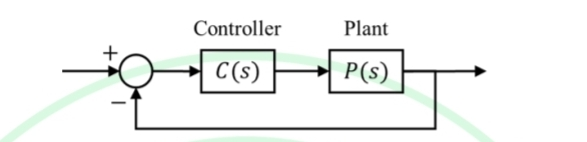
\includegraphics[width=0.6\columnwidth]{Figs/Q-50.jpg}
    \caption{Feedback Control System}
    \label{50}
\end{figure}
\begin{enumerate}
\begin{multicols}{2}
\item proportional (P) controller
\item integral (I) controller
\item proportional-integral (PI) controller
\item proportional-derivative (PD) controller
\end{multicols}
\end{enumerate}


%51
\item Choose the eigenfunction(s) of stable linear time-invariant continuous-time systems from the following options. \par\hfill{\brak{\text{GATE IN 2025}}}
\begin{enumerate}
\begin{multicols}{4}
\item $e^{j \frac{2\pi}{3}t}$
\item $\cos \brak{\frac{2\pi}{3}t}$
\item $2^t$
\item $\sin \brak{\frac{2\pi}{3}t}$
\end{multicols}
\end{enumerate}


%52
\item The probability of a student missing a class is $0.1$. In a total of $10$ classes, the probability that the student will not miss more than one class is \rule{1.5cm}{0.4pt}. (rounded off to two decimal places) \par\hfill{\brak{\text{GATE IN 2025}}}


%53
\item A metallic strain-gauge (SG) with resistance $R_{sg}$ is connected as shown in \figref{53}, where $R_{L1}, R_{L2}, R_{L3}$ represent lead wire resistances. The SG has a gauge factor of $2$ and nominal resistance $R_N=125\,\ohm$. When the SG is subjected to a tensile strain of $2\times 10^{-3}$, the resulting change in $R_{sg}$ is $\Delta R$. The $\Delta R$ value is measured as $\Delta R_{meas}=R_{eq2}-R_{eq1}$. The $R_{eq1}$ and $R_{eq2}$ are the equivalent resistances measured between the terminals 1 and 2, and terminals 2 and 3, respectively. If $R_{L1}=R_{L2}=5\,\ohm$, and $R_{L3}=4.95\,\ohm$, the measured value of tensile strain is \rule{1.5cm}{0.4pt}$\times 10^{-3}$ \brak{\text{rounded off to two decimal places}}. \par\hfill{\brak{\text{GATE IN 2025}}}

\begin{figure}[H]
\centering
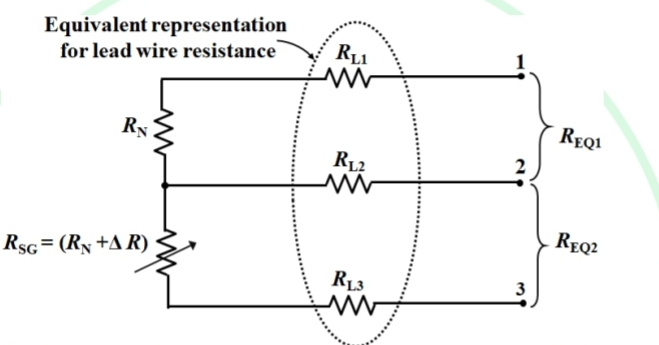
\includegraphics[width=0.6\columnwidth]{Figs/Q-53.jpg}
\caption{Combination of Resistors}
\label{53}
\end{figure}


%54
\item Let $X\brak{e^{j\omega}}$ represent the discrete time Fourier transform of a 4-length sequence $x[n]$, where $x[0]=1,\;x\sbrak{1}=2,\;x\sbrak{2}=2,\;x\sbrak{3}=4$. $X\brak{e^{j\omega}}$ is sampled at $\omega_k=\frac{2\pi k}{3}$ to generate a periodic sequence in $k$ with period $3$, where $k$ is an integer. Let $y\sbrak{n}$ represent another sequence such that its discrete Fourier transform $Y\sbrak{k}$ is given as $Y\sbrak{k} =X\brak{e^{j\omega_k}}$. The value of $y\sbrak{0}$ is \rule{1.5cm}{0.4pt}. \par\hfill{\brak{\text{GATE IN 2025}}}


%55
\item A schematic of a Michelson interferometer, used for the measurement of refractive index of gas, is shown in \figref{55}. The transparent chamber is filled with a gas of refractive index $n_g$ where $n_g \ne 1$, at atmospheric pressure. If a $532$ nm laser beam produces $30$ interference fringes on the screen, then the number of fringes produced by a $632.8$ nm laser beam will be \rule{1.5cm}{0.4pt} \brak{\text{rounded off to one decimal place}}.  
Note: Assume the effect of beamsplitter width negligible. The setup is in air medium with refractive index $=1$. \par\hfill{\brak{\text{GATE IN 2025}}}

\begin{figure}[H]
\centering
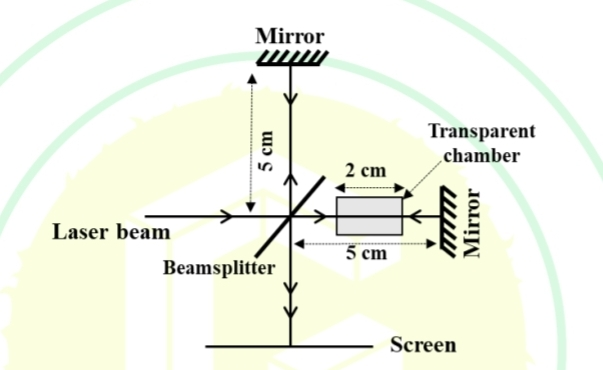
\includegraphics[width=0.6\columnwidth]{Figs/Q-55.jpg}
\caption{Michelson Interferometer}
\label{55}
\end{figure}


%56
\item Consider an AC bridge shown in \figref{56} with $R=300\,\ohm$, $R_1=1000\,\ohm$, $R_2=500\,\ohm$, $L=30$ mH and detector $D$. At bridge balance condition, the frequency of the excitation source $V_s$ is \rule{1.5cm}{0.4pt} kHz \brak{\text{rounded off to two decimal places}}.
\par\hfill{\brak{\text{GATE IN 2025}}}

\begin{figure}[H]
\centering
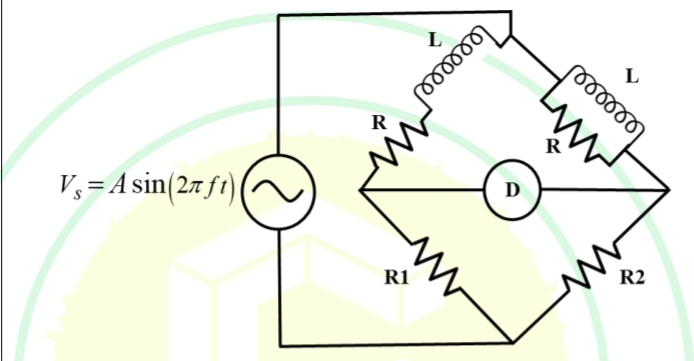
\includegraphics[width=0.5\columnwidth]{Figs/Q-56.jpg}
\caption{AC Bridge Circuit}
\label{56}
\end{figure}



%57
\item An air filled parallel plate electrostatic actuator is shown in the figure. The area of each capacitor plate is $100\,\mu m \times 100\,\mu m$. The distance between the plates $d=1\,\mu m$ when both the capacitor charge and spring restoring force are zero as shown in \figref{57(a)}. A linear spring of constant $k=0.01$ N/m is connected to the movable plate. When charge is supplied to the capacitor using a current source, the top plate moves as shown in \figref{57(b)}. The magnitude of minimum charge $Q$ required to momentarily close the gap between the plates is \rule{1.5cm}{0.4pt}$\times 10^{-14}$ C (rounded off to two decimal places).  
Note: Assume full motion is possible and no fringe capacitance. $\epsilon_0=8.85\times 10^{-12}$ F/m, $\epsilon_r=1$.  \par\hfill{\brak{\text{GATE IN 2025}}}

\begin{figure}[H]
\centering
\begin{subfigure}{.5\columnwidth}
  \centering
  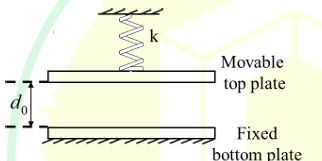
\includegraphics[width=.6\columnwidth]{Figs/Q-57(a).png}
  \caption{Equilibrium State}
  \label{57(a)}
\end{subfigure}
\begin{subfigure}{.5\textwidth}
  \centering
  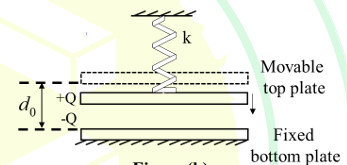
\includegraphics[width=.6\columnwidth]{Figs/Q-57(b).png}
  \caption{Charge is supplied to capacitor}
  \label{57(b)}
\end{subfigure}
\caption{Diagrams for Question-57}
\label{42}
\end{figure}

%58
\item The resistance of a thermistor is measured to be $2.25\,k\ohm$ at $30\degree C$ and $1.17\,k\ohm$ at $60\degree C$. Its material constant $\beta$ is \rule{1.5cm}{0.4pt} K (rounded off to two decimal places). \par\hfill{\brak{\text{GATE IN 2025}}}


%59
\item A feedback control system is shown in \figref{59}.
\begin{figure}[H]
\centering
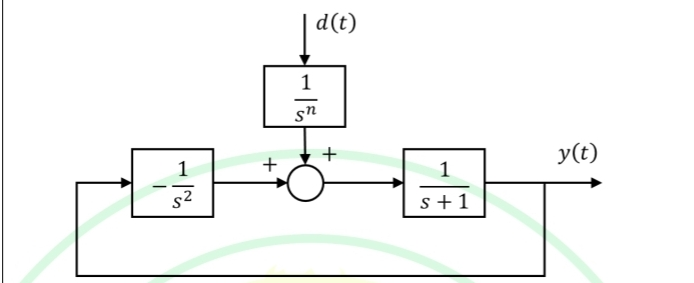
\includegraphics[width=0.5\columnwidth]{Figs/Q-59.jpg}
\caption{Feedback Control System}
\label{59}
\end{figure}
The maximum allowable value of $n$ such that the output $y\brak{t}$, due to any step disturbance signal $d\brak{t}$, becomes zero at steady state, is \rule{1.5cm}{0.4pt}. (in integer) \par\hfill{\brak{\text{GATE IN 2025}}}


%60
\item The circuit given in \figref{60} is driven by a voltage source $V=25\sqrt{2}\angle 30\degree$ V. Operating at a frequency of $50$ Hz, with ideal transformers. The average power dissipated in the $50\,k\ohm$ resistance is \rule{1.5cm}{0.4pt} W (rounded off to two decimal places).
\par\hfill{\brak{\text{GATE IN 2025}}}
\begin{figure}[H]
\centering
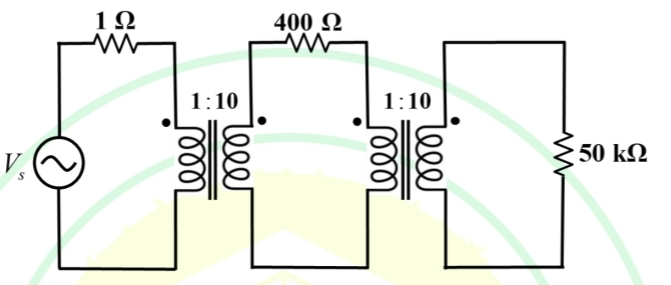
\includegraphics[width=0.6\columnwidth]{Figs/Q-60.jpg}
\caption{Circuit Diagram for Question-60}
\label{60}
\end{figure}


%61
\item In the circuit shown in \figref{61}, the galvanometer $\brak{G}$ has an internal resistance of $100\ohm$. The galvanometer current $I_G=$ \rule{1.5cm}{0.4pt} $\mu A$ \brak{\text{rounded off to nearest integer}}.
\par\hfill{\brak{\text{GATE IN 2025}}}
\begin{figure}[H]
\centering
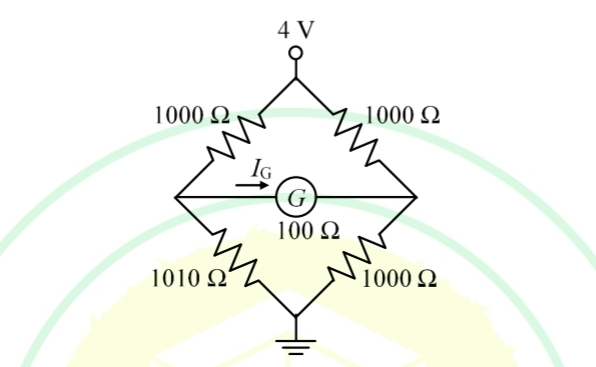
\includegraphics[width=0.5\columnwidth]{Figs/Q-61.jpg}
\caption{Bridge Circuit}
\label{61}
\end{figure}


%62
\item A series RLC circuit resonates at $7500$ rad/s for inductance $L=20$ mH and resistance $R=10\ohm$. The uncertainties in $L$ and $R$ are $0.8$ mH and $0.3\ohm$, respectively. The percentage uncertainty in the measurement of $Q$ is \rule{1.5cm}{0.4pt}\% (rounded off to one decimal place). \par\hfill{\brak{\text{GATE IN 2025}}}


%63
\item In the circuit shown in \figref{63}, the switch is opened at $t=0$ s. The current $i\brak{t=2\,ms}$ is \rule{1.5cm}{0.4pt} mA (rounded off to two decimal places). \par\hfill{\brak{\text{GATE IN 2025}}}
\begin{figure}[H]
\centering
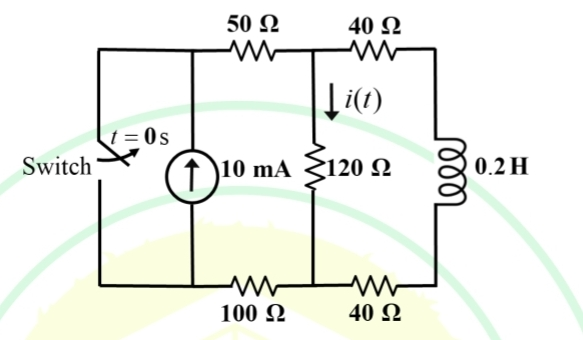
\includegraphics[width=0.6\columnwidth]{Figs/Q-63.jpg}
\caption{Circuit for Question-63}
\label{63}
\end{figure}


%64
\item A signal $v_M=5\sin\brak{\frac{\pi}{3}t}$ V is applied to the circuit consisting of a switch $S$ and capacitor $C=0.1\,\mu F$, as shown in \figref{64}. The output $V_x$ is fed to an ADC having $10\,M\ohm$ in parallel with $0.1\,\mu F$. If $S$ is opened at $t=0.5$ s, the value of $V_x$ at $t=1.5$ s will be \rule{1.5cm}{0.4pt} V (rounded off to two decimal places). \par\hfill{\brak{\text{GATE IN 2025}}}
\begin{figure}[H]
\centering
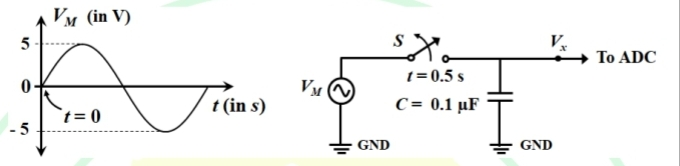
\includegraphics[width=0.8\columnwidth]{Figs/Q-64.jpg}
\caption{Circuit and Graph for Question-64}
\label{64}
\end{figure}


%65
\item For the circuit shown in \figref{65}, the active power supplied by the source is \rule{1.5cm}{0.4pt} W (rounded off to one decimal place.
\par\hfill{\brak{\text{GATE IN 2025}}}
\begin{figure}[H]
\centering
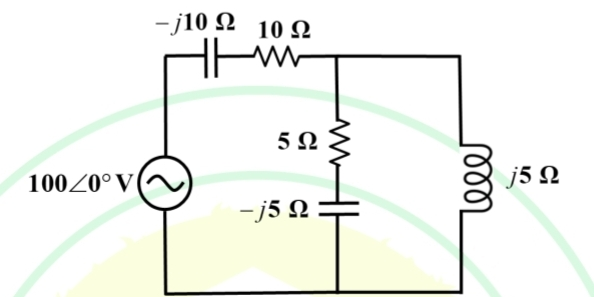
\includegraphics[width=0.5\columnwidth]{Figs/Q-65.jpg}
\caption{Circuit for Question-65}
\label{65}
\end{figure}

\end{enumerate}

\end{document}











